\chapter*{Заключение}                       % Заголовок
\addcontentsline{toc}{chapter}{Заключение}  % Добавляем его в оглавление

%% Согласно ГОСТ Р 7.0.11-2011:
%% 5.3.3 В заключении диссертации излагают итоги выполненного исследования, рекомендации, перспективы дальнейшей разработки темы.
%% 9.2.3 В заключении автореферата диссертации излагают итоги данного исследования, рекомендации и перспективы дальнейшей разработки темы.
%% Поэтому имеет смысл сделать эту часть общей и загрузить из одного файла в автореферат и в диссертацию:

Основные результаты работы заключаются в следующем:
%% Согласно ГОСТ Р 7.0.11-2011:
%% 5.3.3 В заключении диссертации излагают итоги выполненного исследования, рекомендации, перспективы дальнейшей разработки темы.
%% 9.2.3 В заключении автореферата диссертации излагают итоги данного исследования, рекомендации и перспективы дальнейшей разработки темы.
\begin{enumerate}
  \item На основе анализа поставленного задания была выполнена работа по подбору частей, сборке, программированию и тестированию робота;
  \item Эксперименты на ручном управлении показали, что робот отлично выполняет поставленные команды и не имеет проблем с задержкой их выполнения;
  \item Эксперименты с полуавтоматическим управлением показали, что одометрия всё ещё требует улучшений, так как алгоритм SLAM часто прибегает к автокоррекции местоположения на карте на основе показаний облака точек LiDAR;
  \item Для выполнения поставленных задач была изучена область робототехники, которая не изучалась по ходу курса обучения в университете. 
\end{enumerate}

Таким образом была разработана система управления и формирования поведенческой стратегии автономного мобильного робота на основе визуального анализа окружающего пространства. Изображения готового робота можно увидеть на Рисунке~\cref{fig:done}.

\begin{figure}[ht]
    \begin{minipage}[b][][b]{0.32\linewidth}\centering
        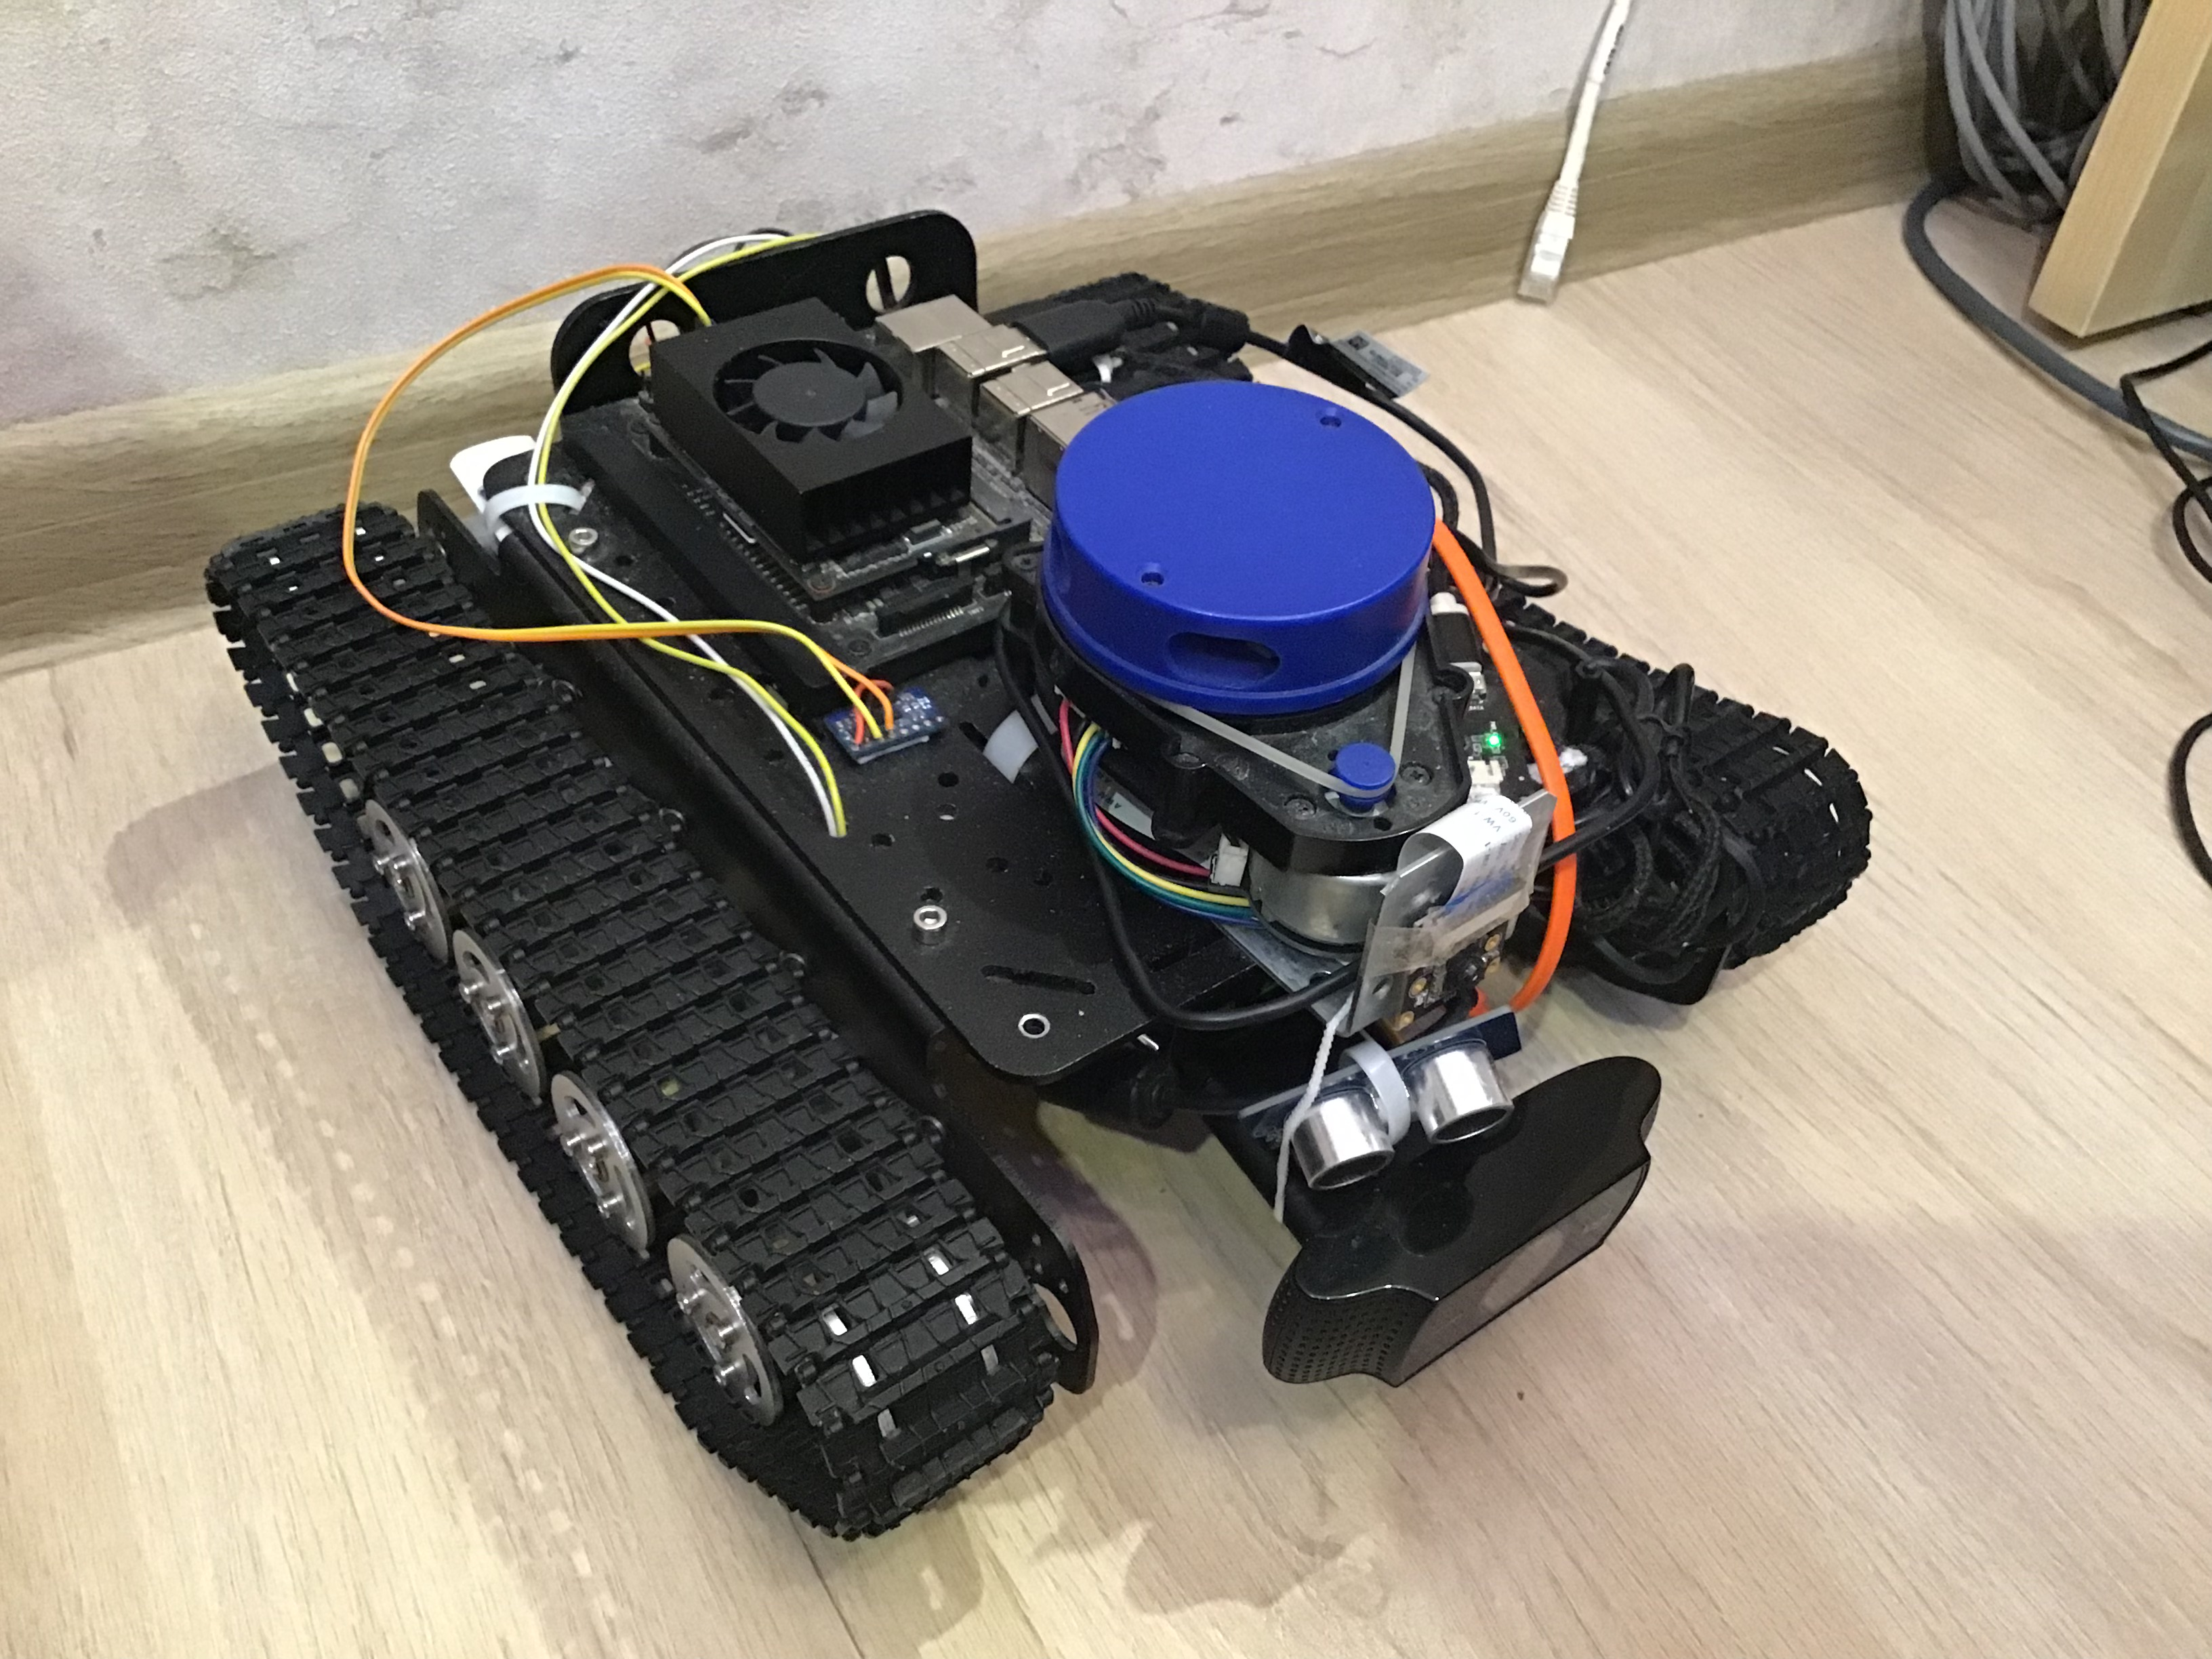
\includegraphics[width=1.0\linewidth]{robot1} \\ а)
    \end{minipage}
    \hfill
    \begin{minipage}[b][][b]{0.32\linewidth}\centering
        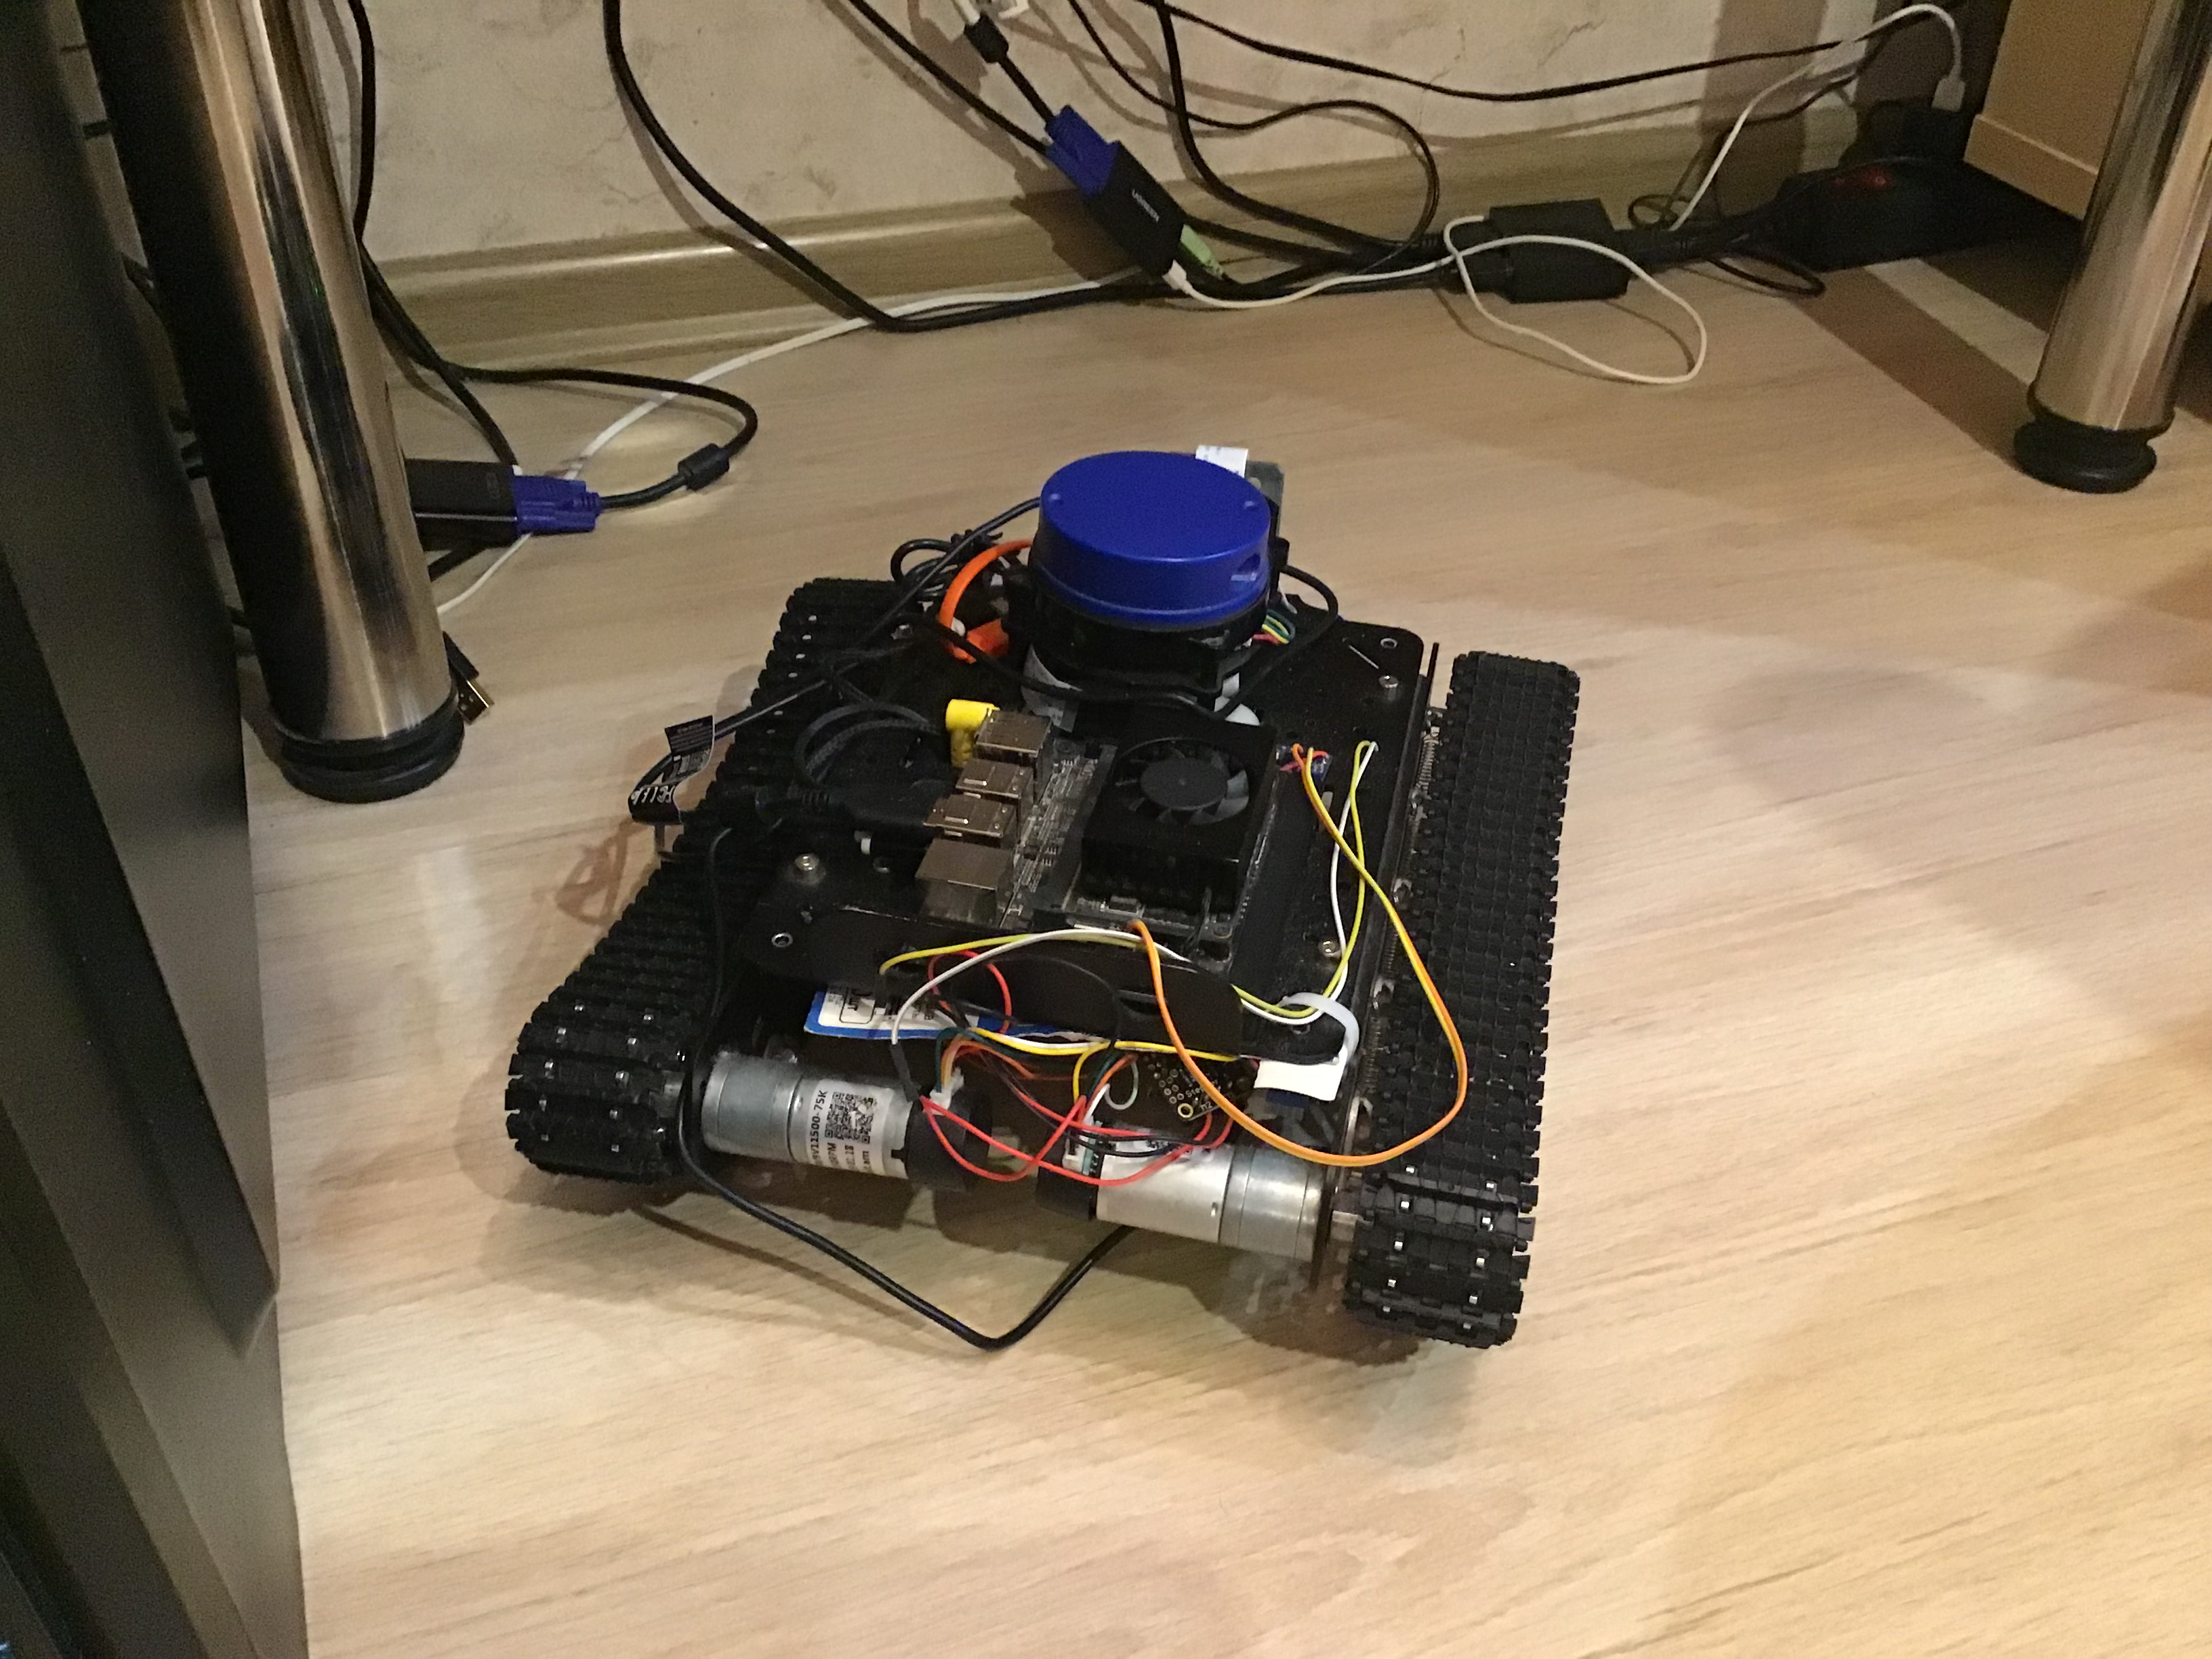
\includegraphics[width=1.0\linewidth]{robot2} \\ б)
    \end{minipage}
    \hfill
    \begin{minipage}[b][][b]{0.32\linewidth}\centering
        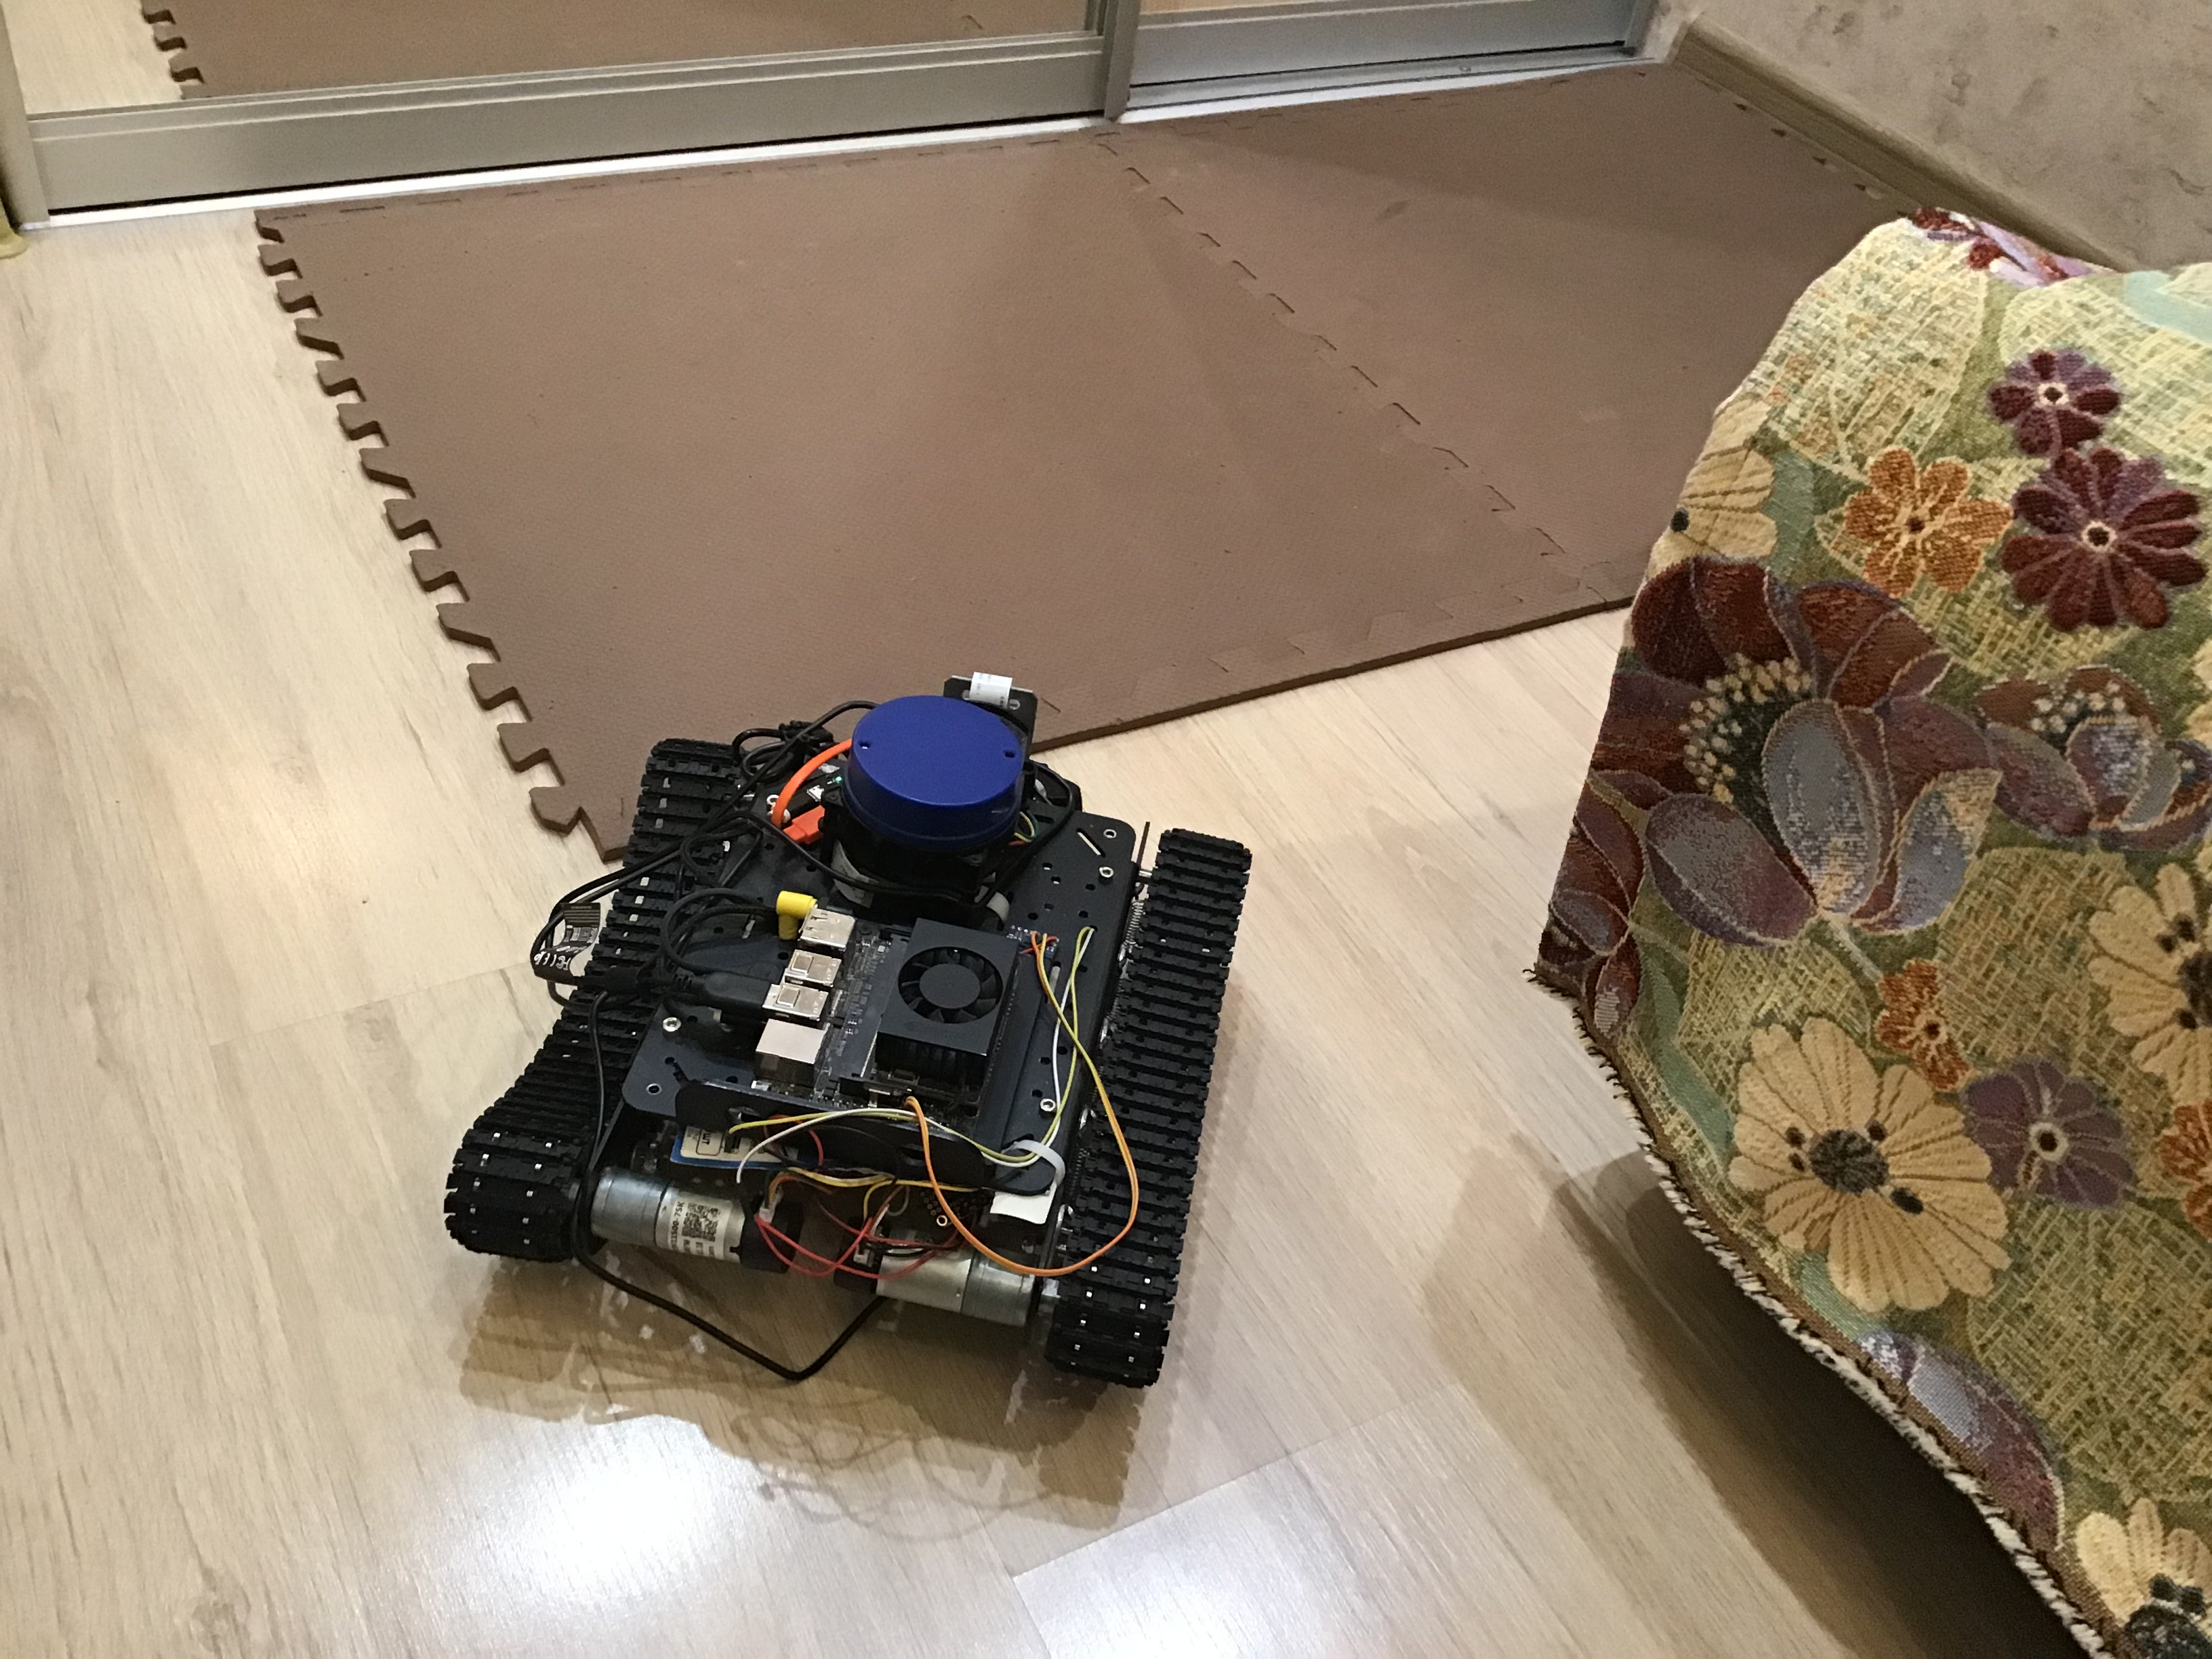
\includegraphics[width=1.0\linewidth]{robot3} \\ б)
    \end{minipage}
    \caption{Готовый робот, выполняющий поездку на полуавтоматическом управлении}
    \label{fig:done}
\end{figure}

В заключение автор выражает благодарность и большую признательность научному консультанту Гордееву~А.\,Ю. и научному руководителю Клячину~В.\,А. за поддержку, помощь, обсуждение результатов и~научное руководство. Также автор благодарит своего коллегу Дряба~А.\,Ю. за посильную помощь при работе с роботом, организатора практики от университета~Полубоярову~Н.\,М. за консультацию при~оформлении работ и авторов шаблона *Russian-Phd-LaTeX-Dissertation-Template* за~свободное распространение своего труда, помогающего оформлять диссертации и выпускные работы. Автор также благодарит много разных людей и~всех, кто сделал настоящую работу автора возможной.
